The most popular advertisement blocking system today is an internet browser plugin called AdBlock Plus. AdBlock Plus works by cross checking internet content with filter lists which tell it if content is an advertisement or not. Any content that it determines to be an advertisement is not displayed to the user\cite{adblock}. Essentially this is how blacklist systems work and is how many existing systems are implemented.

\begin{figure}[h!]
  \caption{AdEater Architecture}
  \label{adeaterimg}
  \centering
    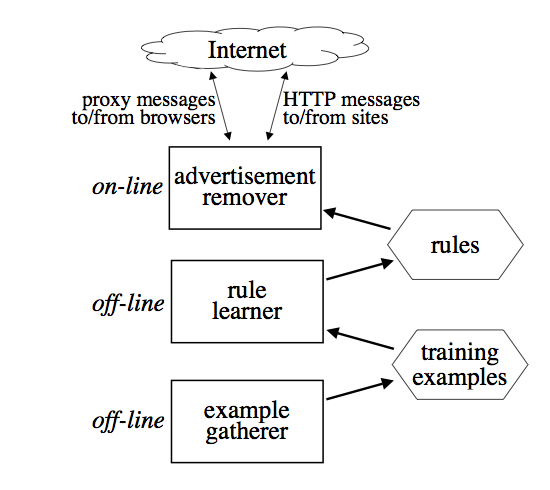
\includegraphics[width=0.5\textwidth]{Figures/adeater.png}
\end{figure}

An advertisement blocking system that functioned using machine learning techniques was previously explored by Nicholas Kushmeric with the development of AdEater. \cite{adeater}. Figure  1 shows how data flows through the AdEater system in order to classify internet advertisements. The AdEater trains its machine learning algorithm offline using a 1558 feature dataset which is generated by scrapping the web. The data is now hosted on the UCI Data Repository website\cite{uci} and contains features about the following advertisement properties:
\begin{itemize}
\item Image Geometry
\item URL
\item Text
\end{itemize}
The image geometry features describe the height, width and aspect ratio of the image which is useful for targeting banner and sidebar ads. The URL features relate the URL of the website with the URL of the image and the website to which the image is linking. The URL features were used to determine if the image was hosted outside of the host website or if the image linked to a website  The majority of the features were generated from related text as they contain information about the alt text, caption, and other surrounding words.  

Kushmeric's goal was to train a C4.5 rules learning algorithm offline and allow for almost  instant classification within a web browser. Implementing the algorithm this way allows for a longer training period if the classification time is significantly less. The C4.5 algorithm is a statistical classifier which generates a decision tree that links relavent features to a set of learned rules for an advertisement. Even though this simple algorithm achieved $97.2\%$ accuracy, we believe that acceptable results could be attained with a smaller feature space and that the system could benefit from a more powerful classifier.

